\documentclass[11pt]{article}

\usepackage[margin=1in]{geometry}
\usepackage{amsmath, amssymb}
\usepackage{booktabs}
\usepackage{cancel}
\usepackage{tikz}
\usetikzlibrary{arrows.meta, positioning, calc}
\usepackage{hyperref}

\newcommand{\indep}{\perp}

\title{CSE 5830 --- Homework 3 Hints}
\author{}
\date{}

\begin{document}
\maketitle

These are hints, not answers. Each worked example uses \emph{different}
numbers or a \emph{different} graph from the homework. Read the example, then
apply the same steps to your problem.

% ============================================================
\section*{Problem 1: Noisy-AND}

\paragraph{Start from noisy-OR (Lec 4, slides 28--31).}
Each parent $X_i$ has a ``mechanism'' variable $Z_i$, and
$\lambda_i = P(Z_i = 1 \mid X_i = 1)$, with $Z_i = 0$ whenever $X_i = 0$.
The leak $Z_0$ is always on, with $P(Z_0 = 1) = \lambda_0$. Then
$Y = Z_0 \lor Z_1 \lor \cdots \lor Z_K$ (deterministic OR). So $Y = 0$ only
when \emph{every} mechanism fails, which gives a product:
\[
  P(Y = 0 \mid X_1,\dots,X_K) = (1-\lambda_0) \prod_{i \,:\, X_i = 1} (1-\lambda_i).
\]

\paragraph{Worked example (noisy-OR).}
$K=2$, $\lambda_0 = 0.1$, $\lambda_1 = 0.7$, $\lambda_2 = 0.4$:
\begin{align*}
  P(Y=0 \mid X_1=1, X_2=1) &= (0.9)(0.3)(0.6) = 0.162, \\
  P(Y=0 \mid X_1=1, X_2=0) &= (0.9)(0.3) = 0.27 \quad
    \text{($X_2$ is off, so it contributes no factor).}
\end{align*}
Notice the product runs only over the parents that are \emph{on}. That is
the ``independence of causal mechanisms'' assumption.

\paragraph{Going from OR to AND (De Morgan).}
Your Week 3 notes say noisy-AND is the dual of noisy-OR via De Morgan:
\[
  \lnot(X_1 \land \cdots \land X_K) = \lnot X_1 \lor \cdots \lor \lnot X_K .
\]
Work through these questions:
\begin{enumerate}
  \item In a deterministic AND, which single condition on one parent is
        enough to force $Y = 0$? Compare this with the OR, where one parent
        being on is enough to force $Y = 1$.
  \item So in the noisy-AND, which value of $Y$ plays the role that $Y=1$
        played in noisy-OR? And which value of $X_i$ ``activates'' the
        mechanism $Z_i$?
  \item This means the ``all mechanisms fail'' product is now a product for
        $P(Y = \underline{\ \ } \mid \cdot)$, and it runs over the parents
        with $X_i = \underline{\ \ }$. Write that down, then take the
        complement to get $P(Y=0 \mid \cdot)$.
  \item What does a leak mean for AND? (Hint: $Y$ can come out \emph{wrong}
        even when every parent looks favorable.)
\end{enumerate}

\paragraph{Convention warning.}
Different sources define $\lambda_i$ for noisy-AND differently. Is it the
probability that $X_i$ \emph{succeeds} in contributing to $Y=1$, or the
probability that $X_i=0$ \emph{succeeds} in forcing $Y=0$? Write one
sentence saying which convention you use. Then check your formula against
these limiting cases:
\begin{itemize}
  \item With no leak and all $\lambda_i = 1$, does it reduce to a
        deterministic AND?
  \item When every parent is in its ``favorable'' state, what remains?
        (It should involve only the leak.)
\end{itemize}

\paragraph{Part (b).} Before you plug in numbers, ask which parents are on
and which are off, and which of them appear in the product under your
convention. $\lambda_0 = 0$ tells you something about the leak term. What
does that factor become?

% ============================================================
\section*{Problem 2: Factor product and reduction}

\paragraph{Definition.} $\psi(X,Y,Z) = \phi_1(X,Y)\,\phi_2(Y,Z)$: for each
full assignment $(x,y,z)$, take the $\phi_1$ row that matches $(x,y)$ and
the $\phi_2$ row that matches $(y,z)$, and multiply them. The shared variable
$Y$ must have the \emph{same} value in both lookups.

\paragraph{Worked example (Koller \& Friedman, Fig.~4.3, trimmed to binary).}
\begin{center}
\begin{tabular}{cc|c}
  \toprule $A$ & $B$ & $\phi_1$ \\ \midrule
  1&1&0.5\\ 1&2&0.8\\ 2&1&0.1\\ 2&2&0\\ \bottomrule
\end{tabular}
\qquad
\begin{tabular}{cc|c}
  \toprule $B$ & $C$ & $\phi_2$ \\ \midrule
  1&1&0.5\\ 1&2&0.7\\ 2&1&0.1\\ 2&2&0.2\\ \bottomrule
\end{tabular}
\qquad
\begin{tabular}{ccc|l}
  \toprule $A$&$B$&$C$&$\psi$\\ \midrule
  1&1&1& $0.5\cdot0.5=0.25$\\
  1&1&2& $0.5\cdot0.7=0.35$\\
  1&2&1& $0.8\cdot0.1=0.08$\\
  1&2&2& $0.8\cdot0.2=0.16$\\
  2&1&1& $0.1\cdot0.5=0.05$\\
  2&1&2& $0.1\cdot0.7=0.07$\\
  2&2&1& $0\cdot0.1=0$\\
  2&2&2& $0\cdot0.2=0$\\ \bottomrule
\end{tabular}
\end{center}
Sanity check: $2^3 = 8$ rows, and a factor product does \emph{not} need to
sum to 1.

\paragraph{Reduction (Lec 5, ``Factor reduction'').} To reduce
$\psi$ to the context $B=1$, keep only the rows with $B=1$ and drop the $B$
column:
\begin{center}
\begin{tabular}{cc|c}
  \toprule $A$&$C$&$\psi[B=1]$\\ \midrule
  1&1&0.25\\ 1&2&0.35\\ 2&1&0.05\\ 2&2&0.07\\ \bottomrule
\end{tabular}
\end{center}
\textbf{Normalize or not?} Factor reduction by itself does not normalize.
If you read $\psi(X,Z\mid Y=1)$ as a conditional \emph{distribution}, then
divide by the sum of the kept rows. In this example the sum is $0.72$, so
the rows become $0.347,\ 0.486,\ 0.069,\ 0.097$. You can show both versions
and say which one you mean.

% ============================================================
\section*{Problem 3: Conditionals in a pairwise MN}

\paragraph{Recipe.}
\begin{enumerate}
  \item Write the conditional as a ratio:
        $p(x_i \mid \text{rest}) = \dfrac{p(x_i,\text{rest})}{\sum_{x_i'} p(x_i',\text{rest})}$.
  \item Substitute the factored form. The partition function $Z$ cancels.
  \item Any factor that does \emph{not} contain $x_i$ is the same in the
        numerator and in every term of the denominator, so it cancels.
  \item What is left is the factors that touch $x_i$, normalized over $x_i$.
\end{enumerate}

\paragraph{Worked example (3-node chain $a - b - c$).}
$p(a,b,c) = \tfrac1Z\,\phi(a,b)\,\phi(b,c)$.
\[
  p(b \mid a, c)
  = \frac{\tfrac1Z\phi(a,b)\phi(b,c)}{\sum_{b'}\tfrac1Z\phi(a,b')\phi(b',c)}
  = \frac{\phi(a,b)\,\phi(b,c)}{\sum_{b'}\phi(a,b')\,\phi(b',c)} .
\]
\[
  p(a \mid b, c)
  = \frac{\phi(a,b)\,\cancel{\phi(b,c)}}{\sum_{a'}\phi(a',b)\,\cancel{\phi(b,c)}}
  = \frac{\phi(a,b)}{\sum_{a'}\phi(a',b)} .
\]
Notice that $p(a\mid b,c)$ does not depend on $c$, because $c$ is not a
neighbor of $a$.

\paragraph{For your 4-cycle.} For each $x_i$, ask: which two factors contain
$x_i$? Which two variables are its neighbors? Are you conditioning on
exactly those neighbors? (Compare your answer with the local Markov
property in Problem~4.)

% ============================================================
\section*{Problem 4: Cliques, Gibbs, local Markov, separation}

\paragraph{Definitions (Lec 5).} A \emph{clique} is a fully connected
subset of nodes. A \emph{maximal clique} is a clique that is not contained
in a larger clique. A distribution \emph{factorizes over} $H$ if it is a
product of factors over cliques of $H$. It is enough to use one factor per
maximal clique, since smaller factors can be multiplied into it.

\paragraph{Worked example graph.}
\begin{center}
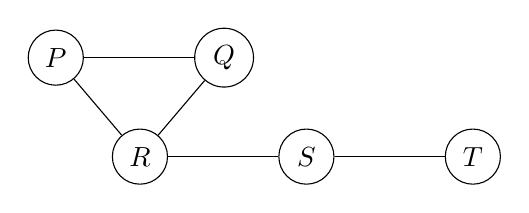
\begin{tikzpicture}[node distance=1.4cm, var/.style={circle,draw,minimum size=7mm}]
  \node[var] (P) {$P$};
  \node[var, right=of P] (Q) {$Q$};
  \node[var, below=0.9cm of $(P)!0.5!(Q)$] (R) {$R$};
  \node[var, right=of R] (S) {$S$};
  \node[var, right=of S] (T) {$T$};
  \draw (P)--(Q); \draw (Q)--(R); \draw (R)--(P); \draw (R)--(S); \draw (S)--(T);
\end{tikzpicture}
\end{center}
\begin{itemize}
  \item \textbf{Cliques:} singletons; the edges $PQ, QR, PR, RS, ST$; the
        triangle $PQR$. (Check: is $QRS$ a clique? No, because there is no
        $Q$--$S$ edge.)
  \item \textbf{Maximal cliques:} $\{P,Q,R\}$, $\{R,S\}$, $\{S,T\}$, so
        $P = \tfrac1Z\,\phi_1(P,Q,R)\,\phi_2(R,S)\,\phi_3(S,T)$.
  \item \textbf{Pairwise MN:} one factor per \emph{edge}, even inside the
        triangle:
        $P = \tfrac1Z\,\phi(P,Q)\phi(Q,R)\phi(P,R)\phi(R,S)\phi(S,T)$,
        with $Z = \sum_{p,q,r,s,t}(\text{same product})$.
  \item \textbf{Local Markov:} each node is independent of everything else
        given its neighbors. For example,
        $P \indep \{S,T\} \mid \{Q,R\}$ and
        $R \indep T \mid \{P,Q,S\}$. Do this for every node.
  \item \textbf{Separation:} Is $P \indep T \mid S$? Every path from $P$
        to $T$ goes through $S$, so yes. Is $P \indep T \mid Q$? No, because
        the path $P - R - S - T$ avoids $Q$.
\end{itemize}

\paragraph{For your graph.} First list every edge carefully. The diagonal
$B$--$F$ edge matters: which triangles does it create? Check each triple
$\{B,?,F\}$. For (d), look for \emph{any} path from $A$ to $F$ whose
interior nodes avoid $\{C, D\}$. One such path is enough to say ``no.''

% ============================================================
\section*{Problem 5: Tree CPDs and context-specific independence}

\paragraph{Reading a tree CPD.} Start at the root and follow the branch
that matches the observed value at each internal node until you reach a
leaf. Variables that are not on that path are \emph{irrelevant} in that
context, even if you were given their values.

\paragraph{Worked example tree.} Leaves are $(P(e^0), P(e^1))$.
\begin{center}
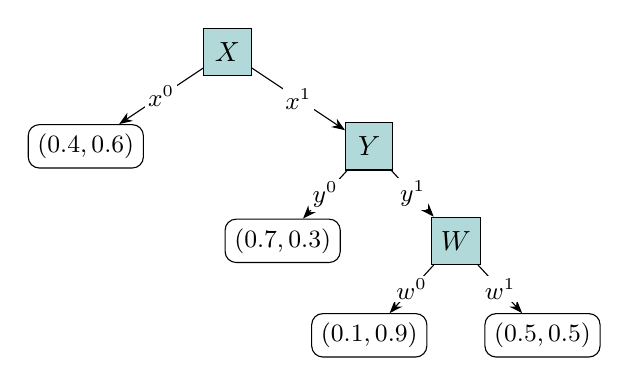
\begin{tikzpicture}[
    level distance=1.2cm,
    level 1/.style={sibling distance=3.6cm},
    level 2/.style={sibling distance=2.2cm},
    inner/.style={rectangle, draw, fill=teal!30, minimum size=6mm},
    leaf/.style={rectangle, draw, rounded corners, font=\small},
    edge from parent/.style={draw, -{Stealth}},
    lab/.style={font=\small, midway, fill=white, inner sep=1pt}]
  \node[inner] {$X$}
    child { node[leaf] {$(0.4,0.6)$} edge from parent node[lab] {$x^0$} }
    child { node[inner] {$Y$}
      child { node[leaf] {$(0.7,0.3)$} edge from parent node[lab] {$y^0$} }
      child { node[inner] {$W$}
        child { node[leaf] {$(0.1,0.9)$} edge from parent node[lab] {$w^0$} }
        child { node[leaf] {$(0.5,0.5)$} edge from parent node[lab] {$w^1$} }
        edge from parent node[lab] {$y^1$} }
      edge from parent node[lab] {$x^1$} };
\end{tikzpicture}
\end{center}
\begin{itemize}
  \item $P(e^1 \mid x^1, y^1, w^0)$: the path is $X\to x^1\to Y\to y^1\to W\to w^0$,
        so the answer is $0.9$.
  \item $P(e^0 \mid x^0, y^1, w^1)$: the path stops right away at
        $x^0$, so the answer is $0.4$. The values of $Y$ and $W$ are ignored.
\end{itemize}

\paragraph{Context-specific independence (Lec 4, slide 16).}
$E \indep_c V \mid c$ means: once the context $c$ is fixed,
$P(E \mid \text{other parents}, V, c)$ is the same for every value of $V$,
\emph{for every setting of the remaining parents}. To check this:
\begin{enumerate}
  \item Mark the branch for the context value in every place it appears in
        the tree. If the context variable appears in several places, mark
        all of them.
  \item Look at every path that is consistent with the context. Does $V$
        appear as a split on any of them?
  \item If $V$ splits on even one consistent path, and its children give
        different leaves, the answer is \textbf{no}.
\end{enumerate}
In the example:
\begin{itemize}
  \item $E \indep_c Y \mid x^0$? \textbf{Yes.} Under $x^0$ there is only a
        leaf, so $Y$ never appears.
  \item $E \indep_c W \mid y^0$? \textbf{Yes.} The paths consistent with
        $y^0$ are $x^0\to$ leaf and $x^1\to y^0\to$ leaf. $W$ appears on
        neither of them.
  \item $E \indep_c Y \mid w^0$? \textbf{No.} $W$ sits \emph{below} $Y$.
        Fixing $w^0$ does not stop $Y$ from mattering on the $x^1$ branch,
        where $y^0$ gives $(0.7,0.3)$ and $y^1, w^0$ gives $(0.1,0.9)$.
\end{itemize}
\textbf{Tip:} fixing a variable that sits \emph{deep} in the tree, or on
only one branch, usually does not remove the influence of variables that
split on \emph{other} branches. Keep this in mind for (e).

\end{document}
